\chapter{Aufgabe D4}

Zur Überprüfung ob es Imbalancen in den Daten gibt, wird das Modell wie in \autoref{fig:drivingdistances1} zu sehen ist erweitert.
Der Mittelwert der vier integrierten Distanzen gilt als Referenzwert um festzustellen, ob ein Reifendruckabfall vorliegt. Die Berechnung ist ebenfalls im erweiterten Modell \autoref{fig:TireSImCurves} zusehen. Anschließend wird die prozentuale Abweichung vom Einzelsignal zum Mittelwert berechnet, weicht die Abweichung um mehr als 0.5\% ab handelt es sich um einen Reifendruckabfall. Die Berechnung ist in \autoref{fig:abweichung1} dargestellt. 
\vspace{-1em}
\begin{figure}[H]
	\centering
	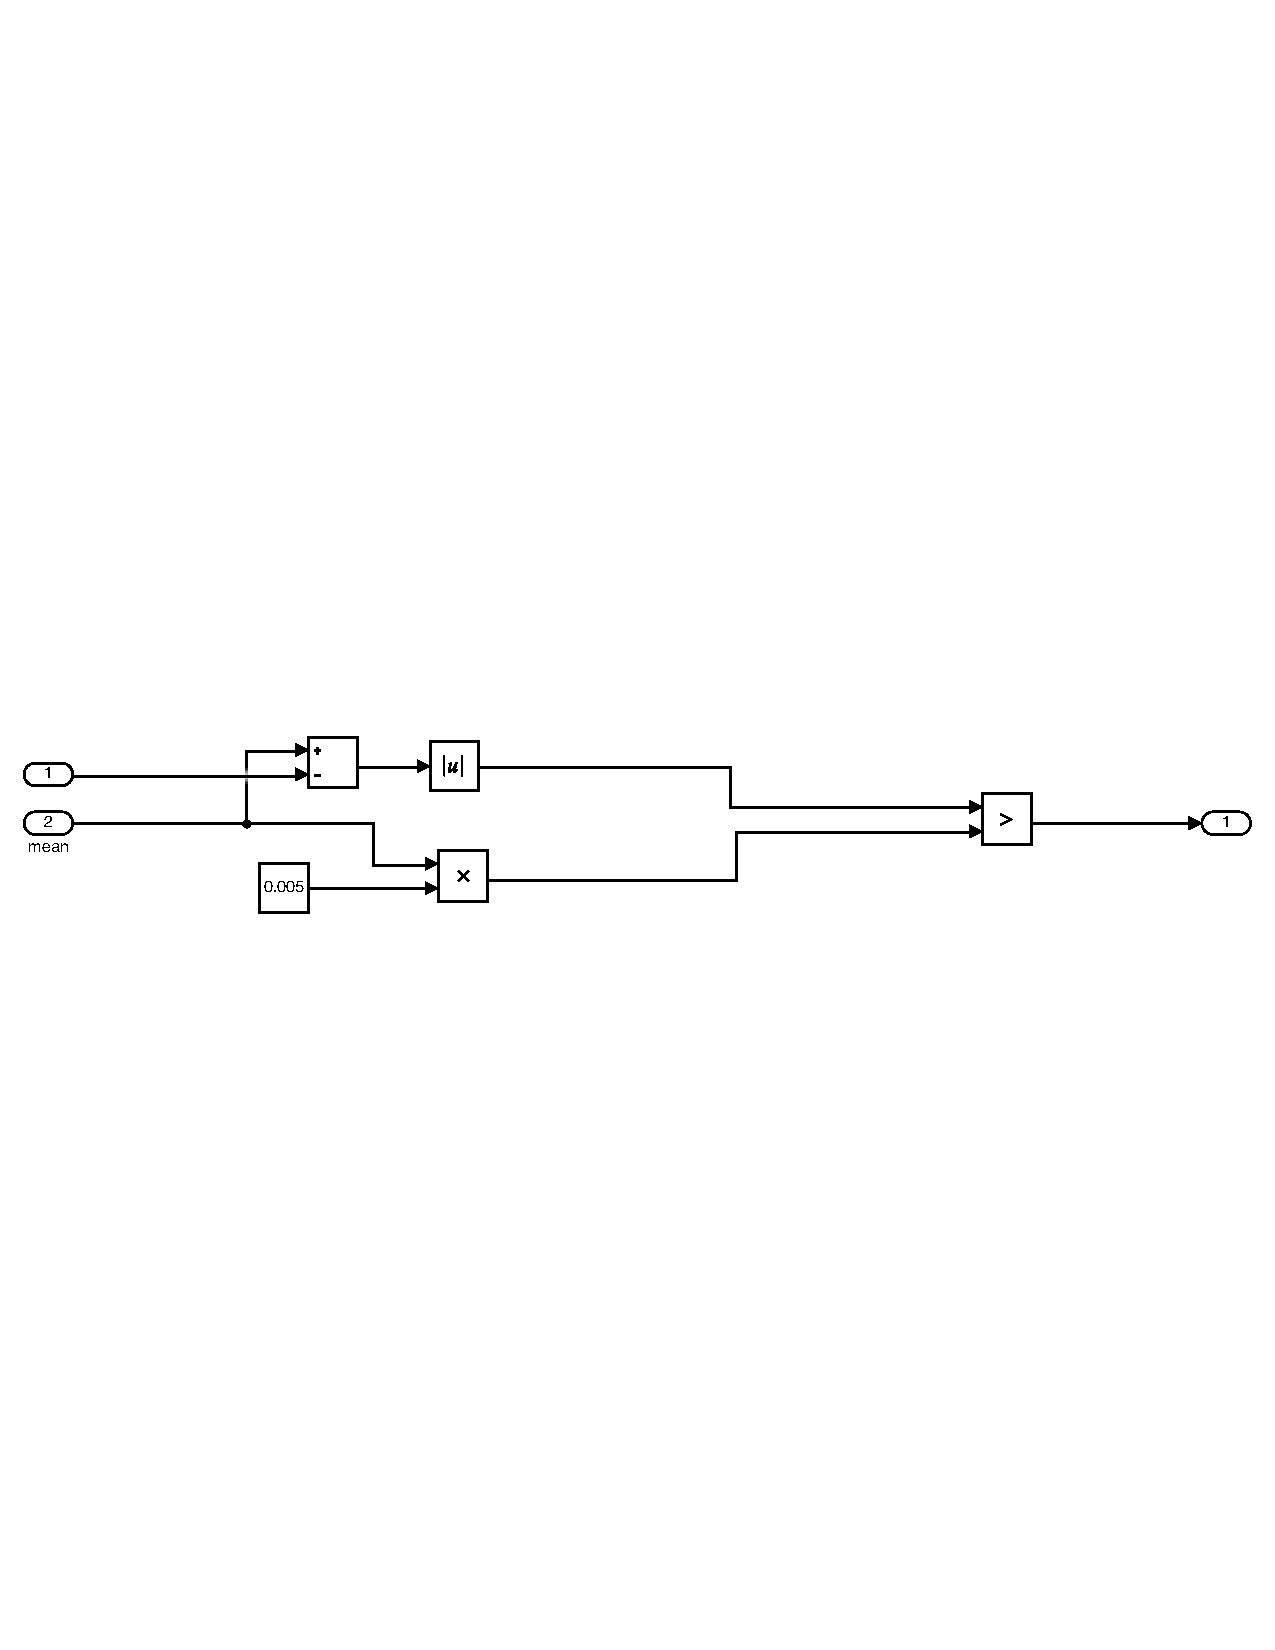
\includegraphics[width=1\linewidth]{../Graphiken/PDFSplit/3_PDFsam_SebastianTireSim2.pdf}
	\caption{Prozentuale Abweichung nach R2}
	\label{fig:abweichung1}
\end{figure}
\vspace{-1em}
Damit die Messungen nicht durch Rauschen im Geschwindigkeitssignal verfälscht werden, wird das integrierte Signal zur Messung verwendet. Durch die Integration wird kurzzeitiges Rauschen sozusagen gemittelt, sodass es die Messung nicht verfälscht. Damit jedoch ein Reifendruckabfall nicht untergeht, da das bereits integrierte Signal zu lange kein Reifenfehler enthielt, wird ein  \glqq Transport Delay"' Block genutzt der das Signal um eine beliebige Zeit (hier 10 Sekunden) verzögert. Das verzögerte Signal kann dann vom Originalsignal abgezogen werden, sodass ausschließlich das Integral der letzten 10 Sekunden betrachtet wird.\footnote{In den ersten 10 Sekunden, ist der Output des Transport Delays 0, sodass in den 10 Sekunden Rauschen durchaus die Messungen verfälschen kann. Deswegen wird der Output des Transport Delays in den ersten 10 Sekunden manuell auf -1000 gesetzt, sodass die Messung in den ersten 10 Sekunden bewusst so manipuliert wird, dass es keine Imbalancen gibt }\\
Die Berechnungen für die Abweichungen werden für jeden Reifen einzeln durchgeführt und anschließend, wie in \autoref{fig:TireSImCurves} zu sehen, verodert, um ein Überblick über das Gesamtsystem zu erhalten.\\


\begin{figure}[H]
	\centering
	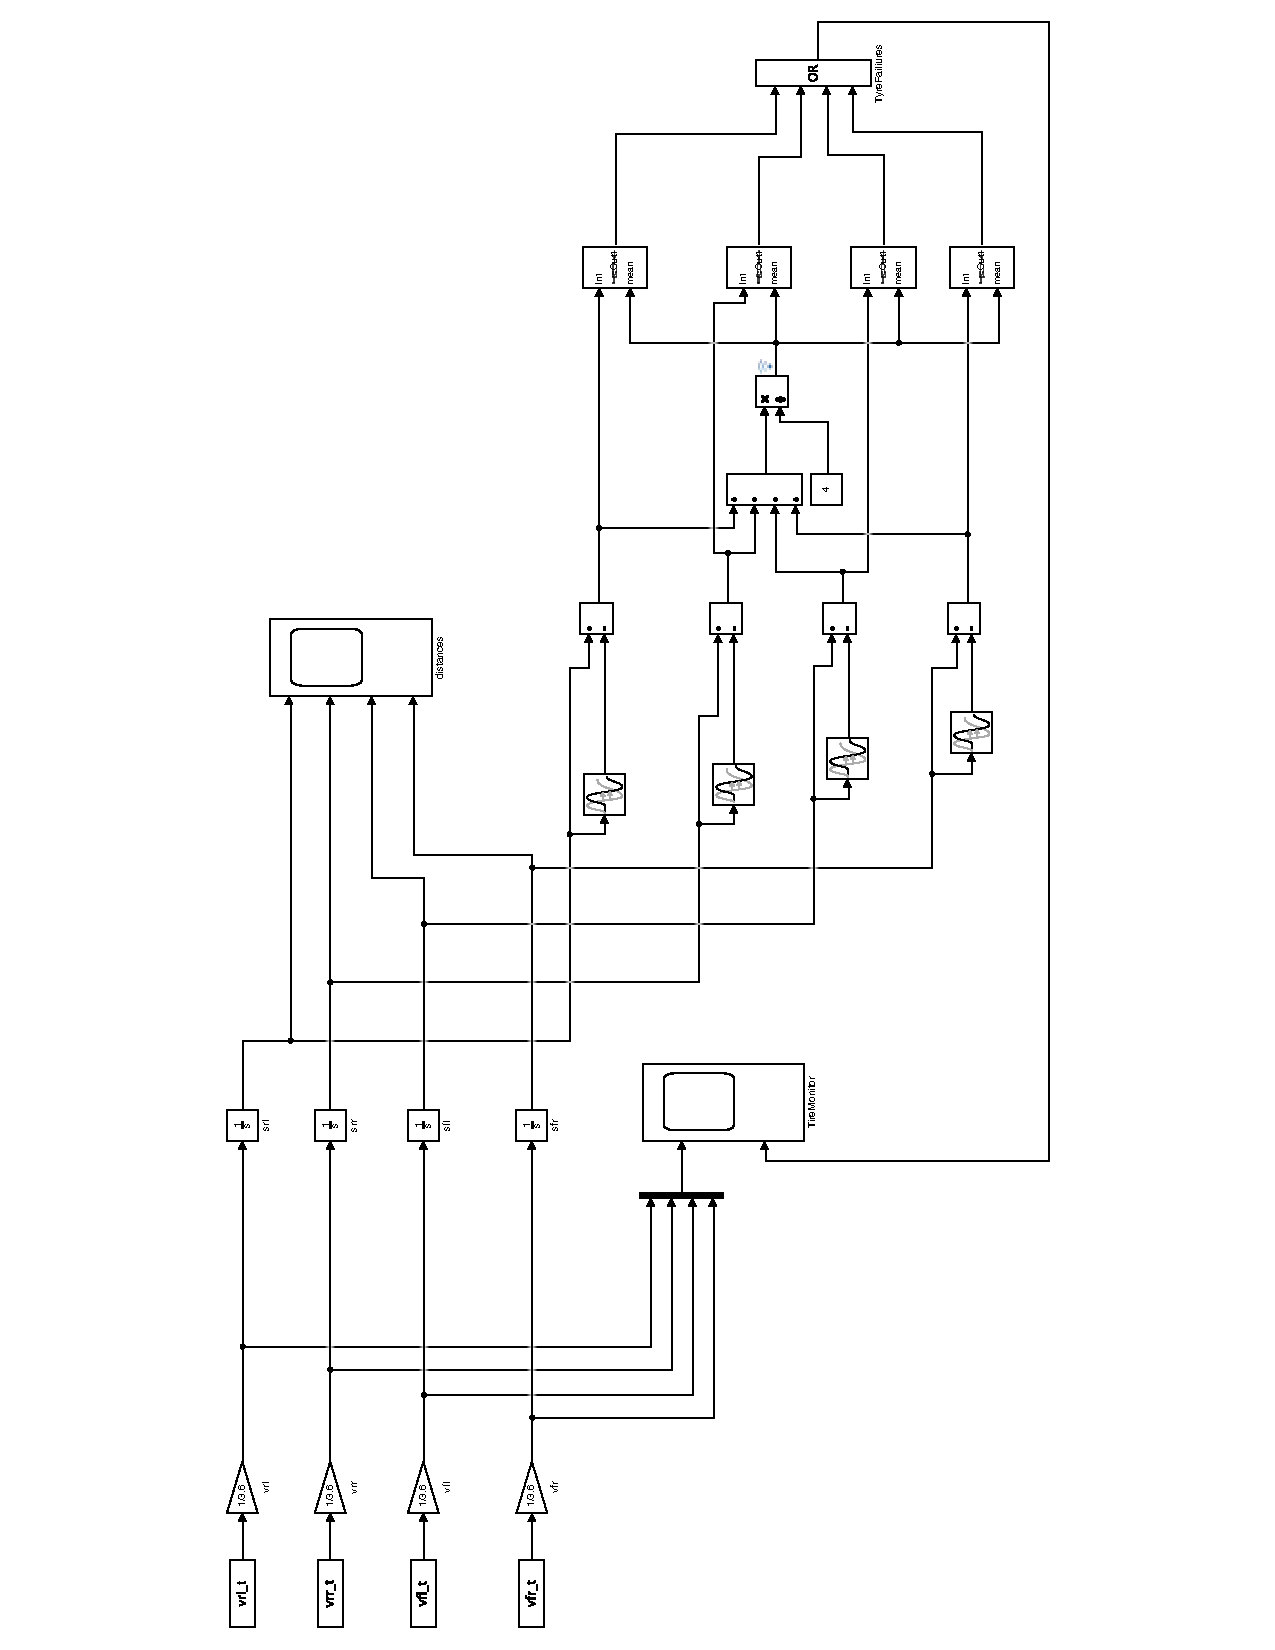
\includegraphics[height=0.95\textheight]{../Graphiken/TireSimCurvesLandscape.pdf}
	\caption{Simulink-Gesamtmodell}
	\label{fig:TireSImCurves}
\end{figure}

%
%Für die Kurvenfahrt entsteht die folgende Datenaufzeichnung über die Reifendruckabweichungen.
%\begin{figure}[H]
%	\centering
%	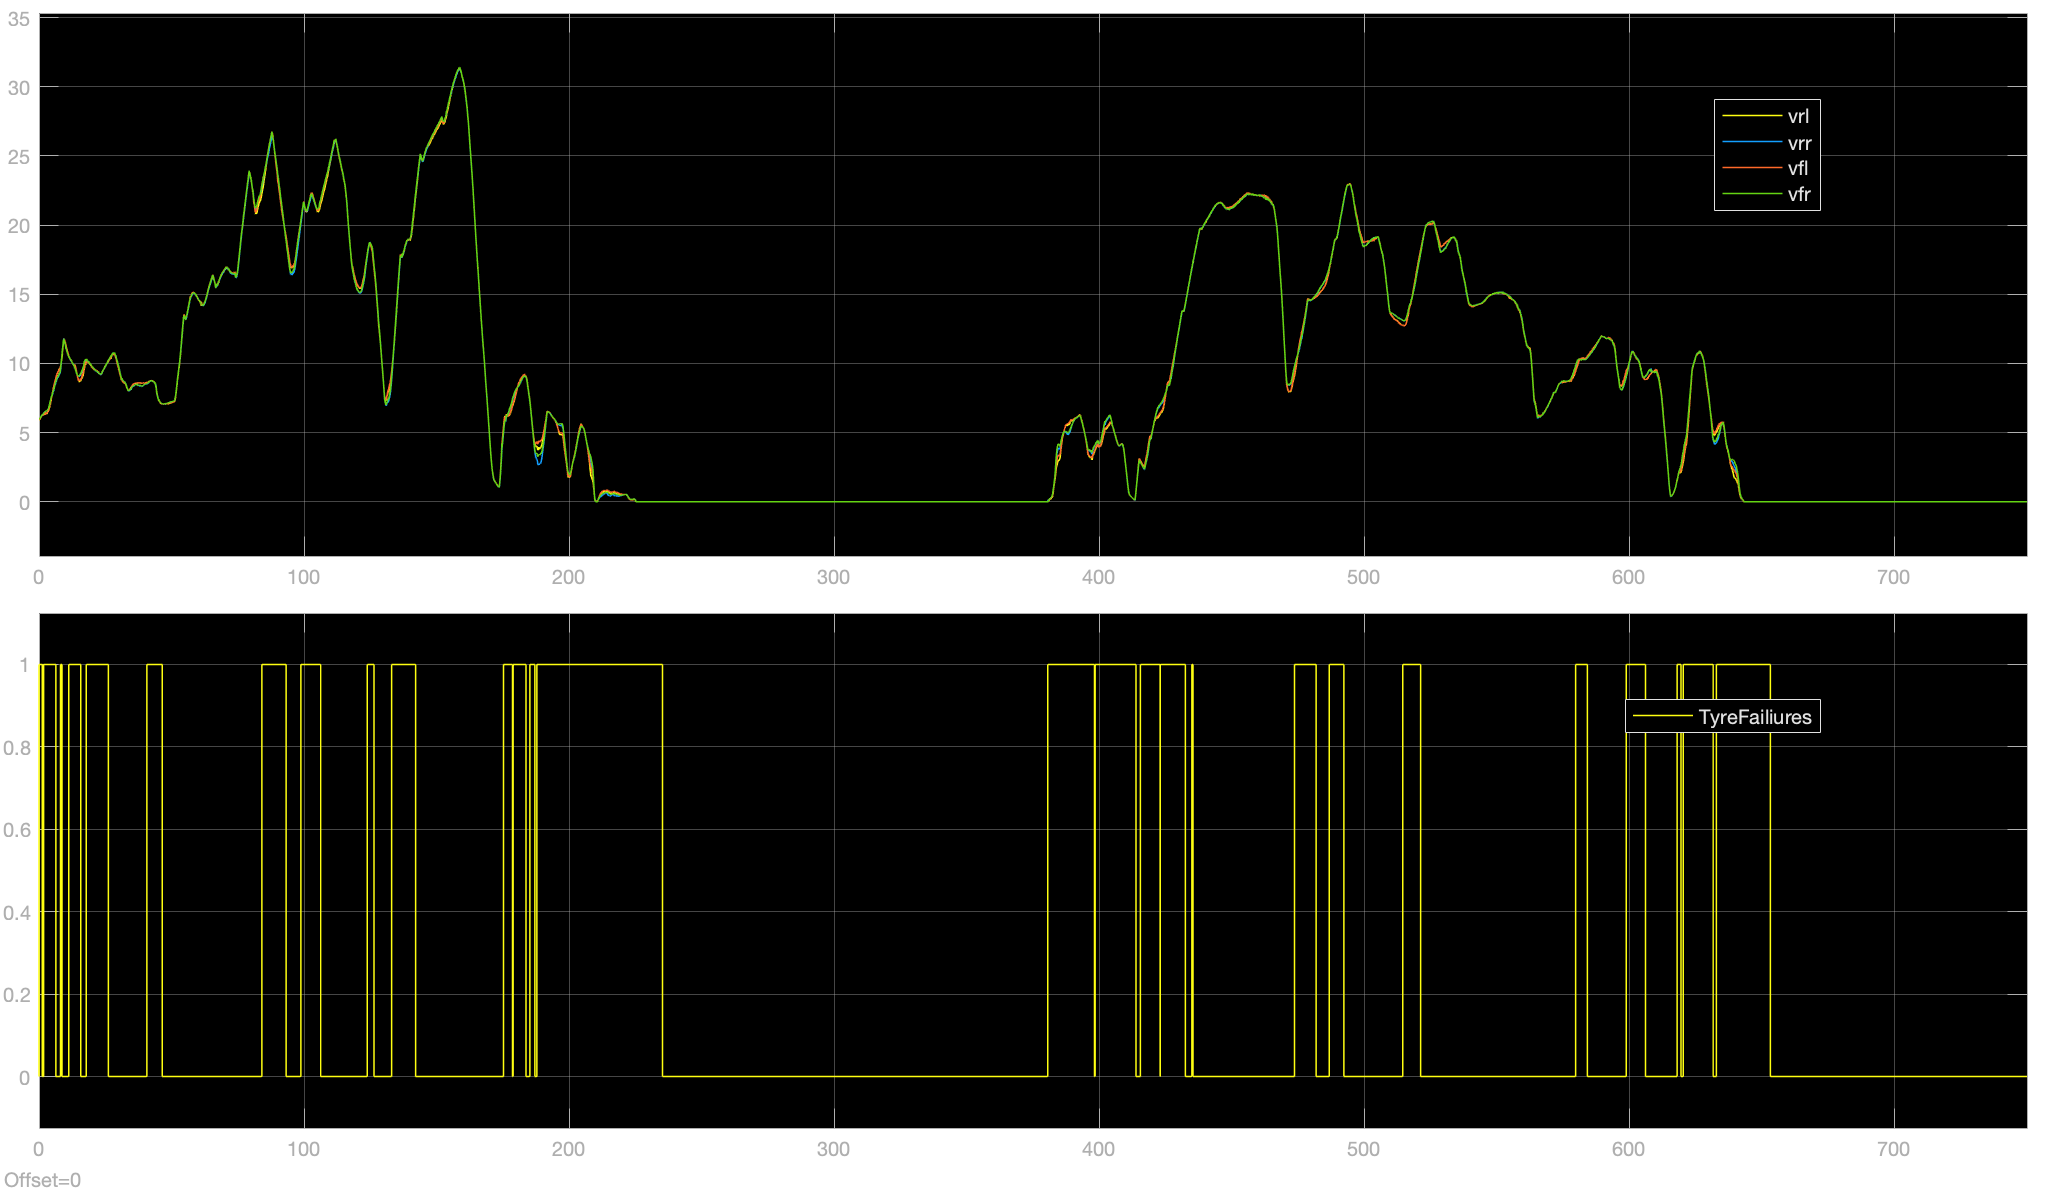
\includegraphics[width=0.95\linewidth]{../Graphiken/CurvesTireMonitor.png}
%	\caption{Tire Monitor für Kurvenfahrt}
%\end{figure}
%Ein Wert von 1  entspricht einer Beobachtung einer Imbalance und ein Wert von 0 entspricht keiner Anomalie.
%\\
%Es werden viele Imbalancen gemessen, aber diese Implementation ist auch nicht für Kurvenfahrten geeignet. Weitere Ausführungen dazu finden bezüglich D13 statt.
%
%


	
	